
\documentclass{article}
\usepackage{csvsimple}
\usepackage{amsmath}
\usepackage{amssymb}
\usepackage{graphicx}
\usepackage{hyperref}
\usepackage{wrapfig}

\begin{document}

%insert your content here..

\section{Student content}
\include{jcastanonremy}
%\documentclass[article]{IEEEtran}
%\usepackage[utf8]{inputenc}
%\usepackage{graphicx}
%\usepackage{cite}
%\usepackage{url}

\title{GitHub Assignment}
\author{Noah Rodgers}
\date{September 2022}

%\begin{document}

\maketitle

\section{About Me}

Hello, my name is Noah Rodgers I am a Graduate Student in the Master of Cyber Security program at UCCS. I work at the Aerospace Corporation as an intern Cyber Specialist working with NASA and the Space Force. What I hope to gain from this course is how to properly conduct my research. As well as write my papers with the correct language and grammar. I hope this will further my research work as I start my work for Dr. Chang. I am working on disrupting satellite communications using different methods examining viability, and effectiveness. I am also hoping that this course will touch on how to write and prepare my thesis for my master’s program. Something personal about me is that I love to go sand boarding at the Great Sand dunes. I also like to long board to class from my home on sunny days although I’m not that good at it but I haven’t crashed yet, so I guess that’s a plus. I got my Bachelors in Game design and Development at UCCS and got my minor in computer science so I’ve been working on filling in the gaps for cyber security. I look forward to what this class has to offer.



\begin{figure}[!htb]
    \centering
    \includegraphics[width=85mm, angle=90]{Me1.jpg}
    \caption{\textbf{Picture of Myself}}
\end{figure}


\section{Git Code}
A collection of Resources for budding SAT hackers (Satellites, not the test¯\_(ツ)_/¯).

This is the basic hack a sat github repo where you can learn and train to help better security for these devices.

https://github.com/deptofdefense/hack-a-sat-library

\section{2 Questions to answer}
How different is the attack vector when facing a hacking process aiming for satellites? - Jose Remy

Not very different although the problem we face in satellites is security vs time. Meaning that older satellites are still up above us floating around still being used for missions and for everyday use. This saves money when we can jsut reuse whats up there already but faces the problem of these systems, these languages they use, the interfaces, their ancient in some terms. Satallite attacks are much like the internet built for acceibility and use rather than security so we see alot of the same attack vectors as any other that would be used.



\bibliographystyle{IEEEtran}
\bibliography{refs}

%\end{document}

\include{AlShami}
% \documentclass{article}
% \usepackage[utf8]{inputenc}
% \usepackage{graphicx}
\graphicspath{ {./images/} }
%\usepackage{hyperref}

\title{Turner  CS600}
\author{James Turner}
\date{September 2022}

%\begin{document}

\maketitle
\newpage
\section{Old Stuff from Assignment 1}
My name is James Turner and I am an active-duty Army Chief Warrant Officer 3 (CW3).  I have served a total of 17 years with 12 years as a Cyber Electromagnetic Warfare (EW) Technician.  This job field is extremely challenging because the technology in the marketplace and capabilities used by our adversaries is constantly changing.  However, it also stimulates innovation and creative thinking and is rewarding when you are part of a team that finds solutions to complex problems.

Recently, I was accepted into the Army’s Advanced Civil School (ACS) program that allows me to attend school full-time and complete a Master’s degree while on active duty.  I have been accepted at UCCS in the Cybersecurity Master of Engineering program, and I am a first term student.  I chose to study cybersecurity because my job field is closely connected with wireless applications and wireless security, and I realized that there is significant job growth in the cybersecurity field.

One of the primary outcomes that I desire from the CS6000 course is to become a more proficient writer and researcher.   I already possess some research and writing skills through my professional military education and on the job experience.  However, military style of writing differs from academia in that the military focuses on a “bottom line up front” perspective and tends to leave details out of formal documents.  I also hope to achieve a greater array of methods that help me conduct more thorough and rigorous research.

Another goal I desire from this course is to enhance my critical thinking.  The military embraces and teaches critical thinking at all levels of leadership education, but I want to gain a greater ability to analyze and test information with scientific methods.  The preponderance of my degree plan and research will be analyzing other tests and scientific data, so I want to be prepared to understand and evaluate those results.  I will need to sharpen my ability to challenge assumptions of others, including myself so that I can become a better researcher.

\begin{figure}
    \centering
    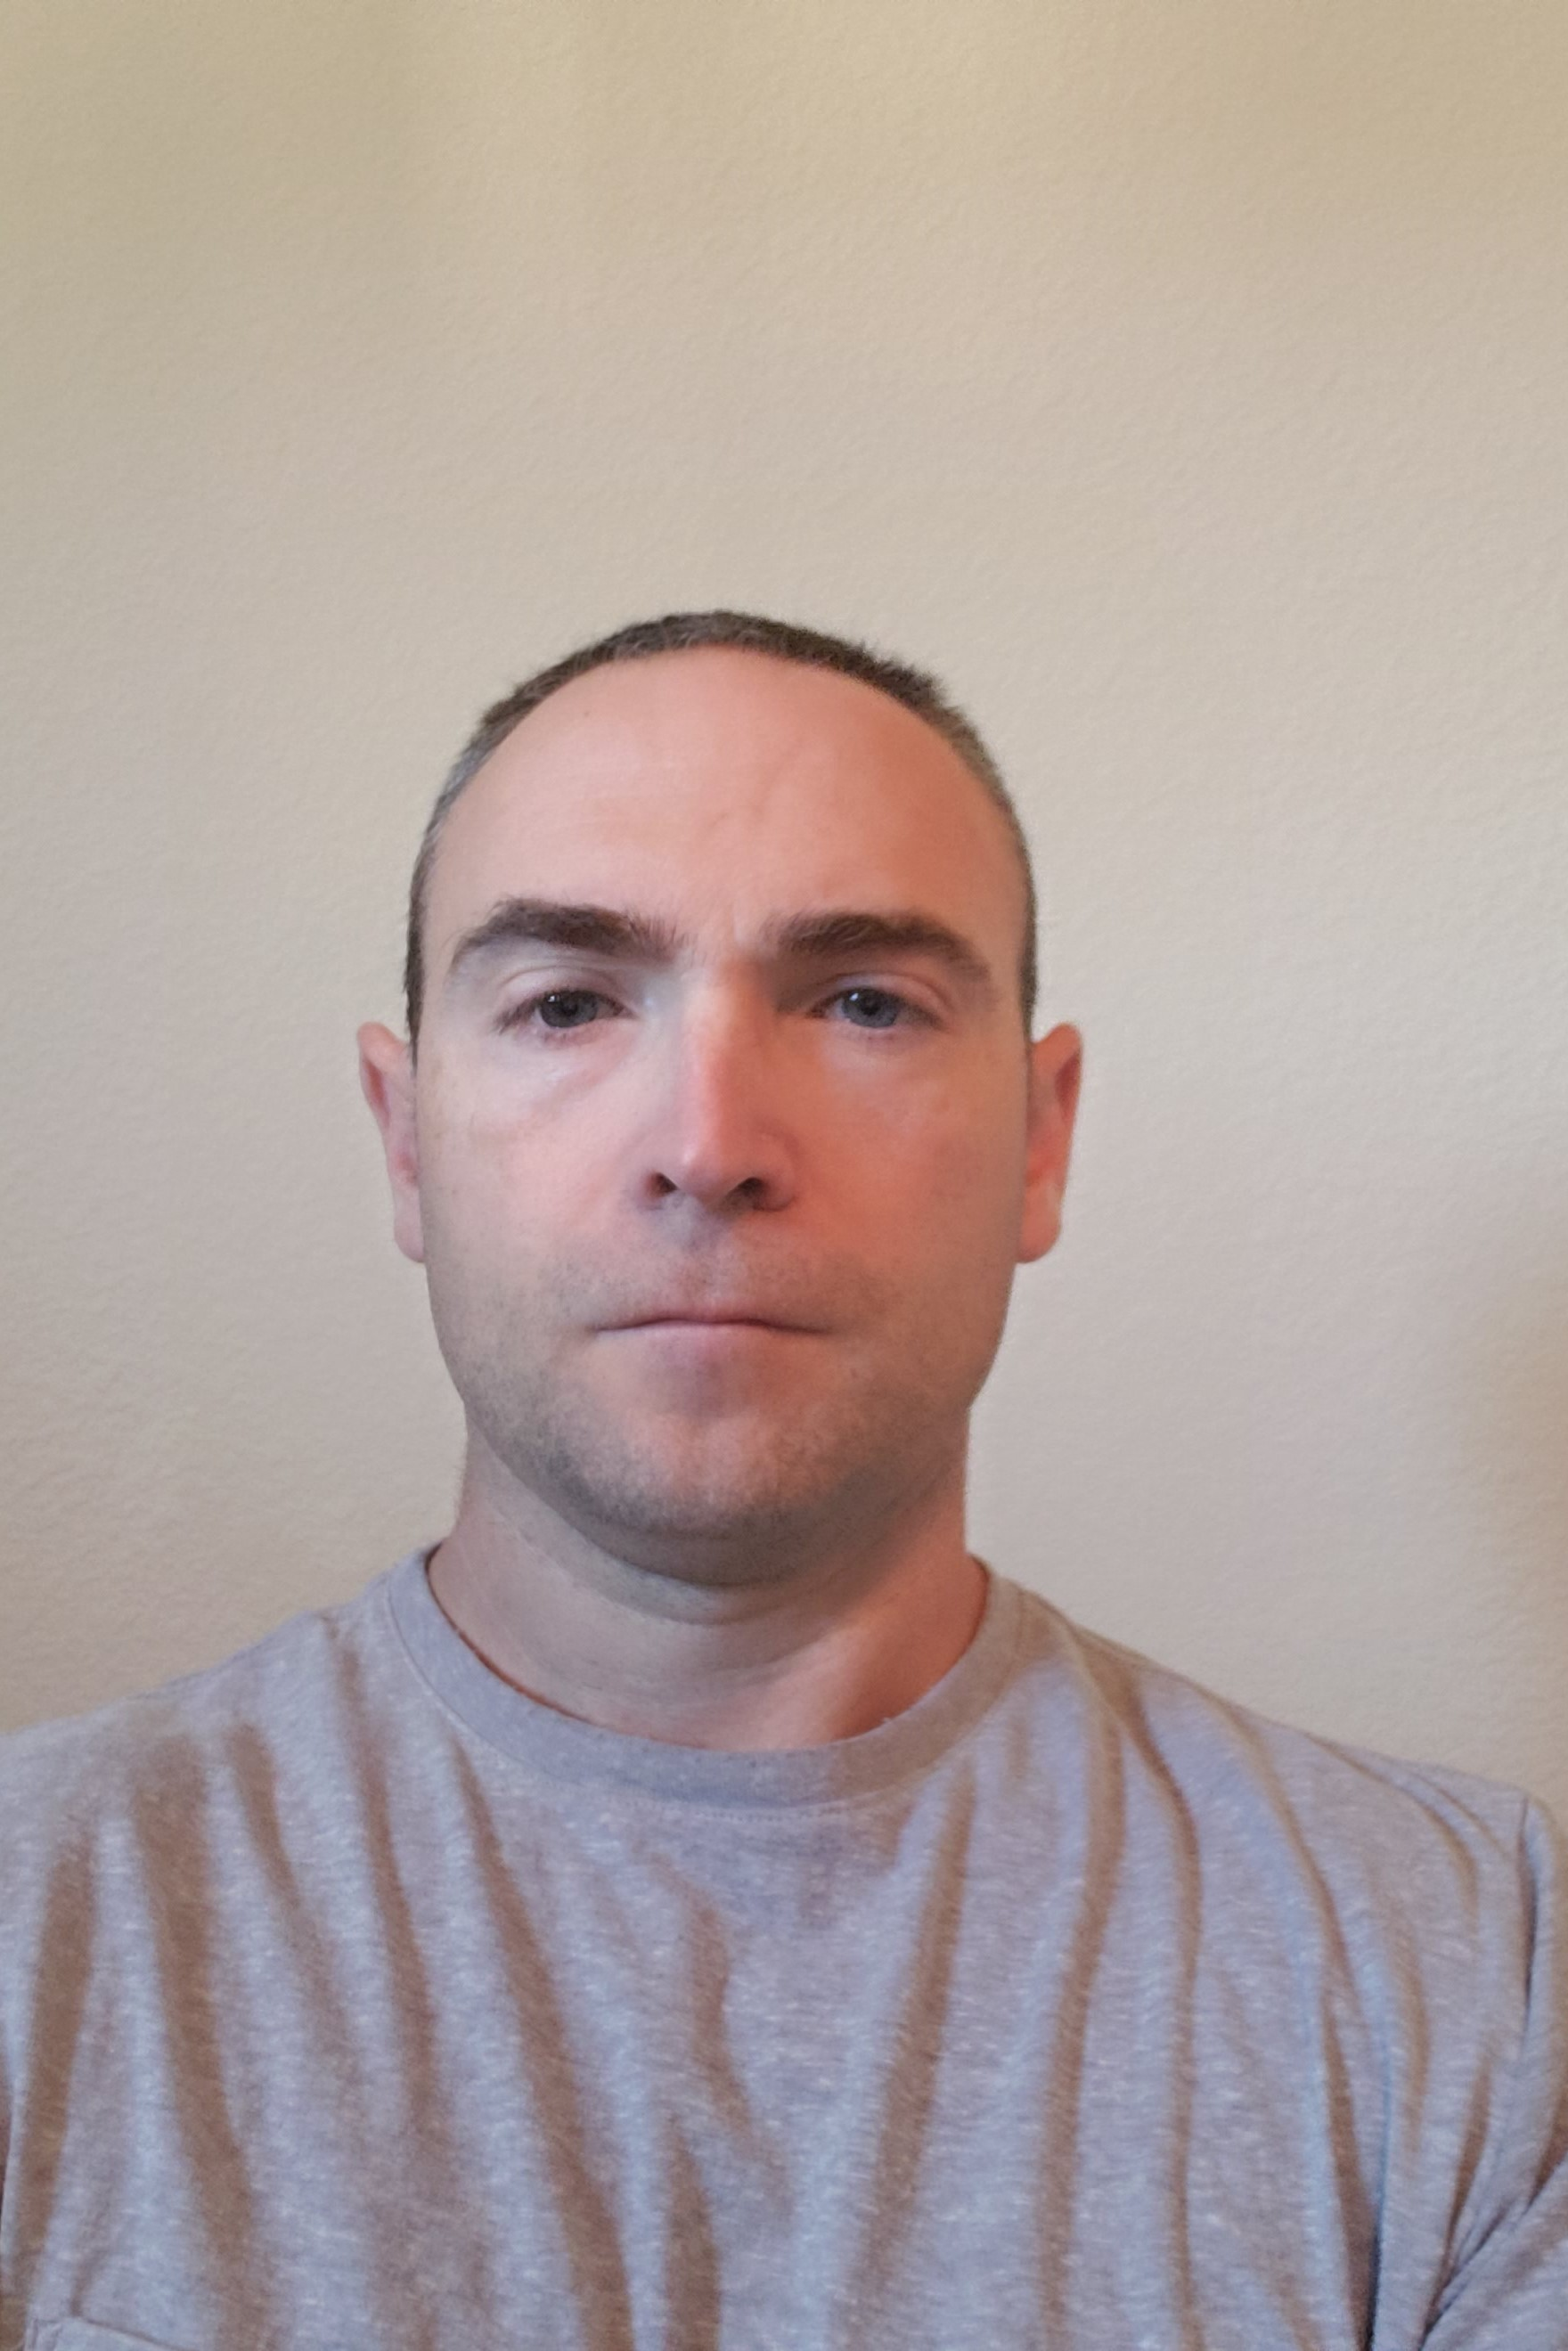
\includegraphics[scale=.1]{self pic2.jpg}
    \caption{me}
    \label{fig:me}
\end{figure}
%\newpage
\section{Github Code on Cognitive Radio}
This repository in Github contains a novel algorithm that uses linear processing to characterize the radio frequency environment in order to enable secondary users' ability to use unoccupied electromagnetic spectrum space.  The link is provided below.
\url{https://github.com/parthgargava/Cognitive-Radio-Networks}

\section{Questions}
What is the main topic that you like to work on for your master thesis, and how do you think that can benefit that army? Ali AlShami
\newline
\paragraph{}
Answer: If I still go the Thesis track then I will discuss some form of wireless security from an avaiability (redundancy and resiliency) and confidentiality perspective.  I still don't know what wireless application I will choose from.  I might focus on 5G or some new type of technology such as reconfigurable intelligent surfaces. 
\paragraph{}
Are you hoping to work on a theoretical or hands-on approach to electronic warfare? I imagine you get a fair share on hands-on experience already. -Katrina
Answer: If I can do live expirementation then that's what I will do.  Yes, I do have plenty of hands-on experiences with different forms of radios and their applications.  However, I need to get stronger from a theoretical standpoint as well.  When you play around with equipment, sometimes it's easy to lose track of the fundamentals in the design of that same equipment.

%\end{document}

%\documentclass{article}

%\usepackage[english]{babel}

%\usepackage[letterpaper,top=2cm,bottom=2cm,left=3cm,right=3cm,marginparwidth=1.75cm]{geometry}


%\usepackage{amsmath}
%\usepackage{graphicx}
%\usepackage[colorlinks=true, allcolors=blue]{hyperref}

\title{Git Assignment}
\author{Hassan Shakil}

\maketitle


\section{Introduction}

Hello, my name is Hassan shakil I am a first year Ph.D. student in UCCS. My major is Computer Science. The reason why I am taking this course in my first semester of the Ph.D. program is that after successfully completing this course I will have knowledge about computer science research and it will help in my Ph.D. degree and also I will get exposure to cutting-edge research in the field which will enable me to explore my passion and abilities. My Research interest in Text summarization using Natural Language Processing. Some personal things about me are that I was an E-sports player in my college team, I love to play and watch soccer. Moreover, I like to explore different places and go hiking.

\begin{figure}[htp]
    \centering
    \includegraphics[width=4cm]{Myimg.jpeg}
    \caption{My picture}
    \label{fig:Myimg}
\end{figure}

\section{Git Code}
To summarize a one-page paragraph in ten sentences, researcher used the NLTK package and techniques including tokenization, stemming, lemmatization, computing similarity, and using the Page-Rank algorithm. Below is the link of git repository that has code related to text summarization.

\url{https://github.com/harshdarji23/Text-Summarization-An-Extractive-Method-NLP.git}

\section{Ask Questions}
Please ask questions here.

Hi Hassan, I'm also interested in natural language processing. Who is your Ph.D. advisor?\\
I looked at the link you provided above. I find the idea really interesting. I liked the synthesis of news to a smaller amount.  There are other services that offer that for news. How do you imagine this could be used, and in how many fields? -- Ken Lee 


Hi Hassan, I'm also interested in natural language processing. Who is your Ph.D. advisor?

Hi, that's great if you are also interested in NLP. My advisor is Dr. Jugal Kalita.

Hassan, I see you are a gamer, what game did you play for E-Sports league?



\include{cardenas}
\documentclass{article}
\usepackage[utf8]{inputenc}
\usepackage{graphicx}
\usepackage{amsmath}
\usepackage{url}
\graphicspath{{./images/}}

\title{CS 6000 Git Assignment}

\author{Katrina J. Rosemond}
\date{September 21, 2022}

%\begin{document}


\section{Introduction - Katrina Rosemond}

Hello, my name is Katrina Rosemond. I am a 3rd year Ph.D. computer science 
student at the University of Colorado Colorado Springs (UCCS). As a 
research assistant in the Embedded Systems Security Lab (ESSL), my 
research focuses on cyber-physical system (CPS) security, particularly 
automotive security. I earned my bachelor's degree in electrical 
engineering from NC A\&T State University. However, I found a passion for 
hardware and software, leading me to pursue a computer science graduate 
degree. 

\begin{figure}[ht]
    \centering
    \includegraphics[width= 1in, height= 1.5in]{RosemondGrad.jpg}
    \caption{Photo of the author, Katrina Rosemond.}
\end{figure}

By enrolling in CS 6000, I aim to improve my research skills and 
understand who I am as a researcher. While I have been contributing to 
research projects since undergrad, I still struggle when I lead my 
projects. Mainly when writing, I never knew how much writing was involved 
when I first started in tech. So when I have to write a paper, I struggle 
with determining what's a good paper, pulling out the necessary 
information, and delivering that information on paper. But I know that the 
more I practice, the more I become comfortable with something. Therefore, 
I hope that between the lessons and assignments in CS 6000, I will learn 
to become a better scientific writer and more comfortable when I need to 
write a research paper.

\section{Git Repo}
The synCAN git repo \url{https://github.com/etas/SynCAN} is a synthetic 
controller area network (CAN) dataset used for CAN intrusion detection 
systems (IDSs). I'm currently researching the quality of CAN IDS datasets.

\section{Questions}
\textbf{Question 1:}
Hi Katrina, what is your PhD about, what kind of project are you currently pursuing?
\newline
\textbf{Answer 1:} I'm currently working on security mechanisms for automotive networks and while I don't have a specific question ready for my dissertation I plan on continuing my work in this area.  
\newline
\textbf{Question 2:}
Hi Katrina, what is your favorite part of your research on cyber-physical systems?
\newline
\textbf{Answer 2:}
\newline
\textbf{*FOR THOSE WHO WILL ADD TO THE DOCUMENT PLEASE REMOVE THE 'BEGIN' AND 'END' PREAMBLES OR THE REST OF DOCUMENT WILL NOT SHOW*}

\documentclass{article}
\usepackage[utf8]{inputenc}
\usepackage{graphicx}
\usepackage{hyperref}
\title{Introduction To Research}
\author{Omolade Ikumapayi}
\date{August 2022}

\begin{document}

\maketitle

\section{Introduction}

\begin{figure}[h!]
  \centering
  
\includegraphics[width=0.5\textwidth]{omolade_.jpg}
\end{figure}

I am a second-year Ph.D. student in the department of computer science at the University of Colorado, Colorado Springs. I work with Dr.Gedare Bloom at the Embedded System Security Laboratory on real-time systems security. Currently I am investigating scheduling algorithms for automotive applications. My goal for taking Introduction to Research class is to get better at research. I believe research is a process and I want to go through the cycle. I consider myself to be creative as I enjoy designing, yet it can be difficult to put ideas into words, and have a thorough statistical and technical representation through the examination of my ideas.
I hope to explore and understand sophisticated scientific publications through this course, which will assist me to get past my research challenges. As someone who wants to increase the caliber of her research, I am also taking this course to network with others who share my interests.
Finally, I believe that by the end of the class, I will have gained the necessary knowledge, skills, and experience to  maximize my potential. With in-depth research, I hope to improve my understanding of the nuances of Cyber-physical systems and take advantage of the opportunity to be taught by the course coordinator. I intend to contribute to the field by applying my theoretical knowledge and scientific ingenuity.
\section{Git Repository}

\url{https://gitlab.com/ipvs/nesting}
\section{Questions}
\subsection{Question 1}


\subsection{Question 2}
\end{document}

\section{Example of Easy Tables}
\csvautotabular{test.csv}


\section*{Better formated Tables}
    \begin{tabular}{r|r|r}%
    % specify table head
    \bf Time (s) & \bf Rel. time (s)& \bf Y Pos
% use head of csv as column names
    \csvreader{test.csv}{}
% specify selected coloumns here
    {\\\hline\csvcoli&\csvcolii&\csvcolvi}
    \end{tabular}
    \clearpage


\end{document}
